\documentclass[11pt,border=5pt]{standalone}
\usepackage{fontspec}
\setmainfont{cmunrm.otf}[BoldFont=cmunbx.otf,ItalicFont=cmunti.otf,BoldItalicFont=cmunbi.otf]
\usepackage{amsmath}
\usepackage{unicode-math}
\setmathfont{NewCMMath-Regular.otf}
\usepackage{tikz}
\usetikzlibrary{arrows.meta,patterns,angles,quotes}
\begin{document}
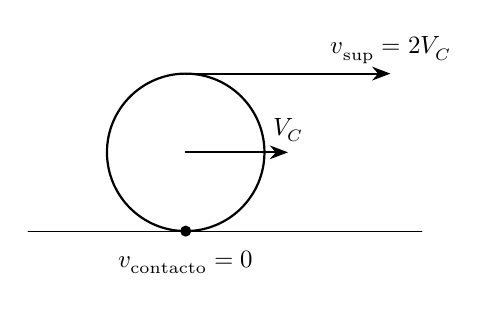
\begin{tikzpicture}[>=Stealth,font=\small,line cap=round,line join=round]
\draw[thick] (0,1) circle(1);\draw(-2,0)--(3,0);\draw[->,thick] (0,1) -- (1.3,1) node[above] {$V_C$};
\draw[->,thick] (0,2) -- (2.6,2) node[above] {$v_{\rm sup}=2V_C$};
\fill(0,0) circle(2pt);\node at (0,-0.4) {$v_{\rm contacto}=0$};

\end{tikzpicture}
\end{document}
